\chapter{Experiment}
\label{cha:experiment}
This chapter discusses an experiment, which compares the performance of the previously described authentication mechanisms.
Even if the performance is not the major decision point to choose the correct authentication mechanism, it is still worth considering it.
Especially, because the migration from a monolithic architecture to the microservice architecture already results in a massive performance decrease of around 79.1\%~\cite{ueda2016workload}.
Therefore the performance is already restricted, and the authentication mechanisms should not produce too much overhead.

\section{Experiment Setup}
The setup consists of two components, the service, that responds to requests and the client, which performs requests and measures the taken time.
Both components are located in the same network and run on the same machine.
The service is developed in C\# using ASP.Net Core, same as the services of the flea market app, mentioned in chapter~\ref{cha:project_structure}.
The client is a console application, developed in C\# using .NET.
It is not a microservice, but it acts as a service that is located within the deployment.
In a usual deployment it is not good practice to access the services directly from an external application, bypassing the API Gateway.
Nevertheless, for the purpose of an experiment, this is allowed to make the setup simpler and reduce falsifications by other components. 

%The experiment consists of two test cases.
%In the first test case (case A), the console application fetches random numbers from the service.
%Therefore the service does not have to establish any connection to a database.
% TODO: geht das nicht besser ?
%The absolute duration of this test case will not be very meaningful, because it is very unrealistic, that a service considers another service for a task like creating a random number.
%But the trend of this times gives a good value for the comparison of the authentication mechanisms, since the falsification of other operations like accessing a database is minimized.
%In the second case (case B), the console application fetches all users stored in a database table.
%The difference between the two test cases will show how much time has is accounted to the authentication mechanisms and how much time is accounted to other tasks.

The experiment simulates the situation that a service (the console application) performs 1000 requests to another service.
The connection between the client and the server has to be established, when the first request is performed.
Therefore the first request will take significantly longer, since the full TCP handshake and TLS handshake have to be performed.
The other request can reuse the already created connection and do not have to perform the whole initialisation process again.
The tests were performed five times to minimize distortions between the test runs.

The console application tracks the whole time, which is needed to perform a request not only the time needed by the service to respond.
This experiment does not aim to give and approximation of the expected request durations with the declared technology stack.
Instead it will compare the trends between the authentication mechanisms.
The exact durations are not relevant, since they are influenced by many factors, like the hardware of the server and the client.

Two different implementations of the approach using self-signed JWTs are demonstrated.
First, an implementation of the self-signed JWT approach, in which a new JWT is created for each request is shown.
The second implementation uses the same JWT for all requests.
This should give an idea how the performance using self-signed JWTs can be improved by efficiently reusing the tokens.
Furthermore the experiment includes the response duration without using any authentication mechanism.
This should show how much time is accounted for the authentication mechanisms and how much time is accounted for other tasks like the transport of the request or the calculation of the random number.

\section{Experimental Results}

\begin{table}[H]
\begin{tabular}{c|cc}
\multicolumn{1}{l|}{\textbf{Authentication Mechanism}} & \multicolumn{2}{c}{\textbf{Average Request Duration}} \\ \hline
\multicolumn{1}{c|}{} & \multicolumn{1}{c|}{first connection} & reuse connection \\ \hline
mTLS & \multicolumn{1}{c|}{$199.66$ ms} & $10.18$ ms \\ \hline
self-signed JWT & \multicolumn{1}{c|}{$226.83$ ms} & $15.38$ ms \\ \hline
self-signed JWT (reusing token) & \multicolumn{1}{c|}{$216.1$ ms} & $8.75$ ms 
%\\ \hline none & \multicolumn{1}{c|}{$216.1$ ms} & $1.71$ ms
\end{tabular}
\caption{Average request durations of the authentication mechanisms, when random numbers are fetched}
\label{tab:experiment_case_1}
\end{table}

The results of the experiment are shown in table~\ref{tab:experiment_case_1}.
As already expected, the approach using no authentication mechanism is the most efficient approach.
The first request takes only ... ms in average and the following requests take only 1... ms in average.
Since the authentication is performed only once per request it is not valid to say that for example the request duration increases by 1018\% when mTLS is used.
The percentual value is only so significant because the task of generating a random number is very simple.
Therefore for this case only the time offsets are interesting.
It shows that the approach using mTLS increases the request duration by about 8ms per request.

The lowest duration for the first connection is achieved using mTLS.
This is reasonable, since the authentication using self-signed JWTs exchanges the certificate of the client in the first request using the extended TLS handshake same as mTLS.
Therefore in all three cases the extended TLS handshake has to be performed but the JWT approaches have to attach the JWT additionally.
The approach that reuses a previously created JWT needs about 10 ms less than the approach in which an new JWT has to be created.
The first connection using an already created JWT takes still around 16 ms more than the first connection using mTLS.
This time overhead is caused by the logic that checks the certificate and stores it into the truststore and then checks the validity of the JWT.

The approach using-self signed JWTs with already created tokens is the most efficient approach that focusing on the requests after the first connection.
Each request takes about 9.7 ms which is about 1.5 ms less than using mTLS.
Nevertheless, the service has to create a new token in some situations. 
Therefore both approaches would have about the same average request durations.
The approach, creating a new JWT for each request has the worst performance.
This shows that the JWT creation takes around 6.5 ms per token in average.

The trend between the request durations is additionally visualized in figure~\ref{fig:trend}.
It shows that the all approaches have a very stable duration timespan except the approach creating a new JWT for each request.

\begin{figure}
	\centering
	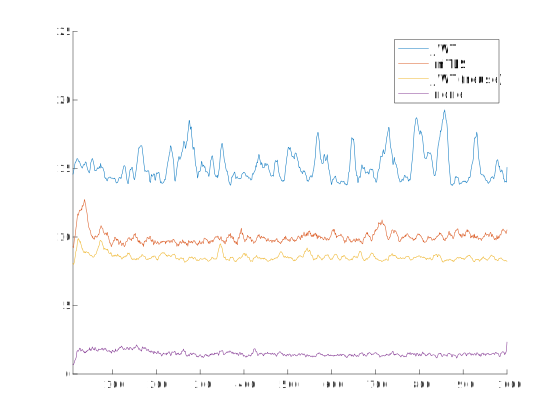
\includegraphics[trim=0 200 0 200, clip, width=\textwidth]{images/experiment/experiment-trend.pdf}
	\caption{Trend of the request duration of the compared approaches excluding the first request}
	\label{fig:trend}
\end{figure}

\section{Conclusion}

